\section{Introduction}
  
    In distributed systems, maintaining the logical clocks of the computers in such a way that they are never too far apart is one of the most complex problems of computer engineering. Whether disciplining computer clocks with the devices synchronized to a (GPS) satellite or a (NTP)\cite{sync4} time server over the Internet, it is possible to equip some primary time servers to synchronize a much larger number of secondary servers and clients connected through a common infrastructure. In order to do this, a distributed network clock synchronization protocol is required through which a server clock can be read, the readings to other clients can be transmitted, and each client clock can be adjusted as required. In such a distributed synchronization approach, the participating devices exchange timing information with their chosen reference at regular intervals and adjust their logical clocks accordingly.\newline
    A computer clock in general has two components, namely a frequency source and a means of accumulating timing events (consisting of a clock interrupt mechanism and a counter implemented in software). The implementation of the computer clock in the operating system and the programming interface differ
    between operating systems and hardware platforms. However, the basic sources of timing errors are an uncompensated quartz crystal oscillator and the clock interrupts it generates. Theoretically, two clocks would remain synchronized if their offsets were set equal and their frequency sources run at the same rate. However,in practice clocks are set with limited precision and the frequency sources run at slightly different rates. In addition, the frequency of a crystal oscillator varies due to the initial manufacturing tolerance, aging, temperature, pressure, and other factors. Because of these inherent instabilities, distributed clocks must regularly be synchronized.
\section{Importance of Time Synchronization}
    Time synchronization is a procedure for providing a common notion of time acrossa distributed system. It is crucial for WSNs when performing a number of fundamental operations, such as \cite{book}:
    \begin{itemize}
        \item Data fusion Data merging is a major operation in all distributed networks for processing and integrating the collected data in a meaningful way, and it requires some or all nodes in the network to share a common timescale.
        \item Power management Energy efficiency is a key factor when designing WSNs since sensors are usually left unattended without maintenance and battery replacement for their lifetimes after deployment. Most energy-saving operations strongly depend on time synchronization. For instance, duty cycling (sleep and wake-up modes control) helps the nodes to save huge energy resources by spending minimal power during the sleep mode. Thus, network-wide synchronization is essential for efficient duty cycling and its performance is proportional to the synchronization accuracy.
        \item Transmission scheduling Many scheduling protocols require time synchronization. For example, the time division multiple access (TDMA) scheme, one of the most popular communications sche
        \item Miscellaneous Many localization, security, and tracking protocols also demand the nodes to timestamp their messages and sensing events.
    \end{itemize}
    Therefore, time synchronization is one of the most important research challenges in the design of energy-efficient WSNs.
    
\section{Signal Models for Time Synchronization}
    \subsection{Definition of Clock}
    Every individual sensor in a network has its own clock. The counter in a sensor is increased in accordance with the zero-crossings or the edges of the periodic output signal of the local oscillator. When the counter reaches a certain threshold value, an interrupt is created and delivered to the memory. The frequency of the oscillator and the threshold value determine the resolution of the clock. Ideally, the clock of a sensor node should be configured such that C (t) = t, where t stands for the ideal or reference time. However, due to the imperfections of the clock oscillator, the clock function of the ith node is modeled as :
    \newline
    \begin{equation}
        \centering
        \label{eq:clock}
        C_{i}( t ) = \theta + \omega t + \epsilon
    \end{equation}
    \newline
    where the parameters $\theta$ and $\omega$ are called the clock offset (phase difference) and clock skew (frequency difference) see\ref{eq:clock}, respectively, and  $\epsilon$ stands for random noise.\newline
    Assuming the effect of random noise $\epsilon$ is negligible, from \ref{eq:clock}, the clock relationship between two nodes, say node 1 and node 2, can be represented by the following equation :\newline
     \begin{equation}
        \centering
        \label{eq:two_clock}
        C_{i}( t ) = \theta^{'} + \omega^{'} C_{j}(t) \tab[0.3cm] i,j \in N , i \neq j , \epsilon = 0 
    \end{equation}
    \newline
    where $\theta^{'}$and $\omega^{'}$ are the relative clock offset and skew between node i and node j, respectively. Thus, $\theta^{'}$ = 0 and $\omega^{'}$ = 1 when the two clocks are perfectly synchronized see\ref{}cl. Suppose there are L nodes in the network, then the global network wide synchronization is achieved when $C_{j}(t) = C_{i}(t)$ for all i, j $\in \left\{1..L\right\}$ .
    \subsection{Design Considerations}
    Time synchronization for conventional wired networks has been thoroughly studied and a plethora of synchronization protocols have been proposed as surveyed in \cite{sync5}.However, for WSNs, there are a number of unique and important factors to be considered when designing time synchronization protocols as listed next \cite{book} :
    \begin{itemize}
        \item Energy consumption
        \item Latency
        \item Security and reliability
        \item Network topology
        \item Scalability
    \end{itemize}
    \subsection{Delay Components in Timing Message Delivery}
    In WSNs there exist a number of non-deterministic delays while transferring messages between nodes. Kopetz and Ochsenreiter were the first to analyze the structure of message delays and characterized the delay components according to the process of message delivery \cite{delay}. The delay components in message delivery can be categorized as follows \cite{book}:
     \begin{itemize}
        \item Send time
        \item Access time
        \item Transmission time
        \item Propagation time
        \item Reception time
        \item Receive time
    \end{itemize}
    \textbf{Note} that the time delay in message transmission also depends on other factors, such as the hardware platform, the error correction code, and the modulation scheme .


\section{Fundamental Approaches to Time Synchronization}
various protocols targeting clock synchronization in WSNs have been proposed, mainly based on packet synchronization techniques.
In general, this family of protocols can be broadly divided into three fundamental approaches\cite{book}:

		 \subsection{Sender Receiver Synchronization}
		The sender node periodically sends a message with its local time as a timestamp to the receiver and then the receiver synchronizes with the sender using the timestamp received from the sender\cite{book}see \ref{fig:x Receiver_to_receiver}.
		%figure Sender–Receiver Synchronization

   
 
    
    
    \subsection{Receiver receiver synchronization}
	    This method uses the property that if any two receivers receive the same message in a single-hop transmission, they receive it at approximately the same time. Receivers exchange the time at which they received the same message and compute their offset based on the difference in reception times\cite{book} see\ref{fig:x Receiver_to_receiver}.
	    %figure
	     \begin{figure}[h!]
	    	\centering
	    	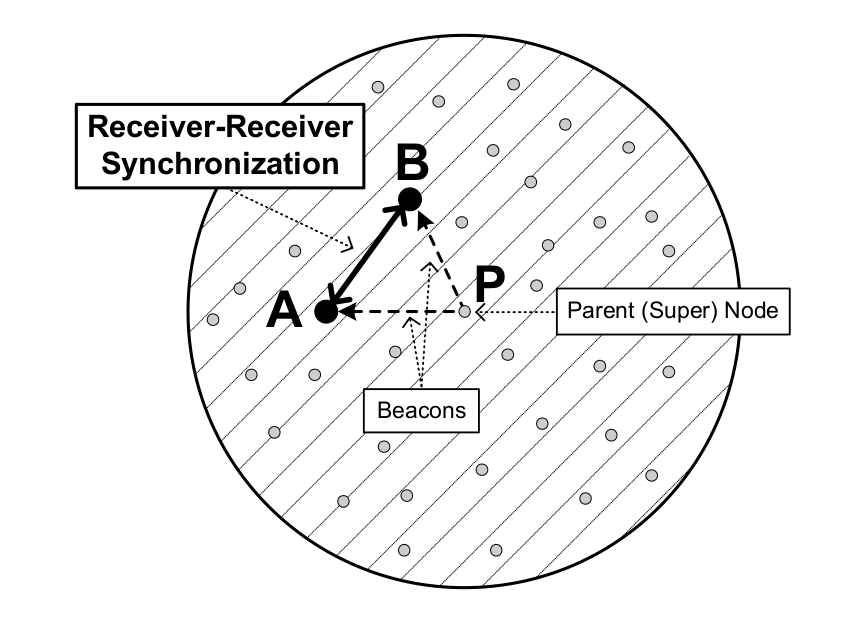
\includegraphics[scale=0.5,width=15cm,height=9cm]{photos/receiver_receiver.png}
	    	\caption{Receiver-receiver synchronizatio}
	    	\label{fig:x Receiver_to_receiver}
	    	
	    \end{figure}
    
    
    
    \subsection{Receiver only synchronization}
	    A group of nodes can be simultaneously synchronized by only listening to the message exchanges of a pair of nodes\cite{book} see\ref{fig:x Receiver_Only}.
	    %figure
	    \begin{figure}[h!]
	    	\centering
	    	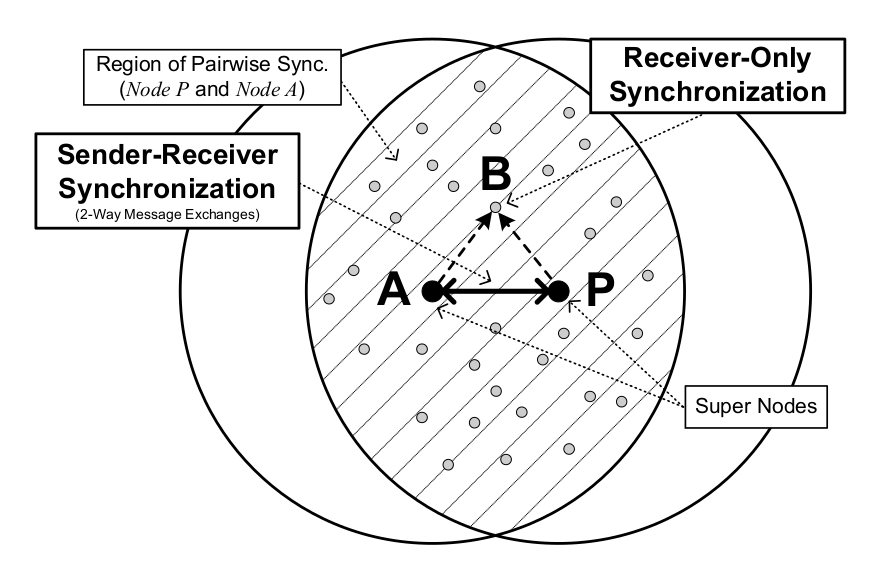
\includegraphics[scale=0.5,width=15cm,height=9cm]{photos/reciverOnly.png}
	    	\caption{Receiver-only synchronization}
	    	\label{fig:x Receiver_Only}
	    	
	    \end{figure}
	    
    
    
    
\section{Time Synchronization Protocols}
A time synchronization protocol should be able to work optimally in terms of all the design requirements imposed on time synchronization in WSNs\cite{book}, which include energy efficiency, scalability, precision, security, reliability, and robustness to network dynamics. However, the complex nature of WSNs makes it very difficult to optimize the protocol with respect to all these requirements simultaneously\cite{book}. Due to the tradeoffs in satisfying these requirements, each protocol is designed to put distinct emphases on different requirements\cite{book}.
\newline Time synchronization protocols can be categorized into following classes :\cite{book}
\begin{itemize}
	\item Master–slave vs. peer-to-peer : 
	\item Clock correcting vs. untethered clock :
	\item Synchronization approach : 
	\item Pairwise synchronization vs. network-wide synchronization :
\end{itemize}


\subsection{Lightweight Tree-Based Synchronization}
The primary goal of the Lightweight Tree-Based Synchronization (LTS) protocol (VanGreunen and Rabaey 2003) is to provide a specified precision (instead of a maximum precision) with as little overhead as possible. LTS can be used with different algorithms for both centralized and decentralized multi-hop synchronization.

\subsection{Timing-sync Protocol for Sensor Networks}
The Timing-sync Protocol for Sensor Networks (TPSN) (Ganeriwal et al. 2003) is another traditional sender–receiver synchronization approach that uses a tree to organize a network. TPSN uses two phases for synchronization: the level discovery phase (executed
during network deployment) and the synchronization phase.
\subsection{Flooding Time Synchronization Protocol}
The goals of the Flooding Time Synchronization Protocol (FTSP) (Maróti et al. 2004) are
to achieve network-wide synchronization with errors in the microsecond range, scalability
up to hundreds of nodes, and robustness to changes in network topology including link
and node failures. FTSP differs from other solutions in that it uses a single broadcast
to establish synchronization points between sender and receivers while eliminating most
sources of synchronization error
\subsection{Consensus-based Multi-hop Time	Synchronization Protocol in Wireless Sensor	Networks}
The Consensus Time Synchronization \cite{sync2} is a novel distributed time synchronization approach which overcomes the shortcomings of centralized and consensus time synchronization schemes by combining their advantages. The timing messages are exchanged following the RO methodology. This reduces the communication overhead and energy consumption and speeds up the convergence time. The sensor nodes compensate their clock offset and skew by synchronizing to multiple synchronized nodes which increases synchronization accuracy and robustness to node failures. In addition, nodes are organized intohierarchical structure, which allows to establish a particular communication pattern between nodes leading to reduce the number of exchanged messages and the convergence time .


